\documentclass[11pt,a4paper]{article}
\usepackage[danish]{babel}
\usepackage{enumitem}
\usepackage{array, tabularx}
\usepackage[table]{xcolor}
\usepackage{colortbl}
\usepackage{unicode-math}
\usepackage{pgfplots}
\usepackage{tikz}
\usepackage{xurl}            
\usepackage[hidelinks]{hyperref}   
\usepackage{lipsum}

\urlstyle{same}                 
\hypersetup{
  colorlinks=true,
  linkcolor=black,
  urlcolor=blue,                
  citecolor=black
}
\urlstyle{same}
\pgfplotsset{compat=1.18}

\setlist[enumerate,1]{
    label=\mbox{},        
    leftmargin=0pt,       
    labelsep=0pt,
    align=left,
    itemsep=1.5\baselineskip 
}
\setlist[enumerate,2]{
    label=(\alph*),
    leftmargin=2em,
    labelsep=.6em,
    itemsep=\baselineskip
}

\title{Aflevering 2.3}
\author{Luis Parker Noah Conradty \& Carl Viggo Riesenhuber Hofman}


\begin{document}
    \maketitle
    \begin{enumerate}
        \item{Opgave 1}
            \begin{enumerate}
                \item
                    \begin{align*}
                        f(x) &= 2x\\
                        g(x) &= ln \left(\frac{e^2}{4}x \right)
                    \end{align*}
                \item
                    \begin{align*}
                        f(x) &= -\frac{1}{3}x + \frac{10}{3}\\
                        g(x) &= \frac{3}{\sqrt[3]{\frac{2}{3}}}·\sqrt[3]{\frac{2}{3}}^x
                    \end{align*}
                \item
                    % Punkter: A(1,3), B(4,2), C(-4,0)
                    Vi søger en parabel
                    \[
                    h(x) = ax^{2} + bx + c
                    \]
                    som går gennem punkterne \(A(1,3)\), \(B(4,2)\) og \(C(-4,0)\).

                    \[
                    \begin{aligned}
                    A(1,3):\quad &h(1)   = a\cdot1^{2} + b\cdot1 + c = 3 
                        &&\Rightarrow a + b + c = 3 \tag{I} \\
                    B(4,2):\quad &h(4)   = a\cdot4^{2} + b\cdot4 + c = 2 
                        &&\Rightarrow 16a + 4b + c = 2 \tag{II} \\
                    C(-4,0):\quad &h(-4) = a\cdot(-4)^{2} + b\cdot(-4) + c = 0 
                        &&\Rightarrow 16a - 4b + c = 0 \tag{III}
                    \end{aligned}
                    \]

                    Fra (II)–(III) får vi
                    \[
                    2 - 0 = (16a+4b+c) - (16a-4b+c)
                    \Rightarrow 2 = 8b
                    \Rightarrow b = \frac14.
                    \]

                    Indsæt \(b = \tfrac14\) i (I) og (II):
                    \[
                    \begin{aligned}
                    (I):\quad & a + \frac14 + c = 3 
                        &&\Rightarrow a + c = \frac{11}{4},\\[2mm]
                    (II):\quad & 16a + 4\cdot\frac14 + c = 2
                        &&\Rightarrow 16a + 1 + c = 2
                        \Rightarrow 16a + c = 1.
                    \end{aligned}
                    \]

                    Nu
                    \[
                    (16a + c) - (a + c) = 1 - \frac{11}{4}
                    \Rightarrow 15a = -\frac{7}{4}
                    \Rightarrow a = -\frac{7}{60}.
                    \]

                    Til sidst findes \(c\) fra \(a + c = \tfrac{11}{4}\):
                    \[
                    c = \frac{11}{4} - a 
                    = \frac{11}{4} + \frac{7}{60}
                    = \frac{43}{15}.
                    \]

                    Dermed er forskriften
                    \[
                    {h(x) = -\frac{7}{60}x^{2} + \frac14 x + \frac{43}{15}}.
                    \]


            
            \end{enumerate}
        \item{Opgave 2}
            \begin{enumerate}
                \item 
                    \(A\) er længden den forskydes fra ligevægtspositionen\\
                    \(ω\) er frekvensen\\
                    \(ϕ\) er forskydningen i tiden \\
                    \(R\) er fjederlængden i hvilepositionen\\
                \item
                    $A$ får værdien 8, fordi det er Amplituden. 4,8 kommer fra $2π$ dividered med $ω$, hvilken er 1,3.
                    $\fracπ2$ betyder at det starter med Amplituden og ikke i hviletilstandet.

                    \begin{figure}[htbp]
                        \centering
                        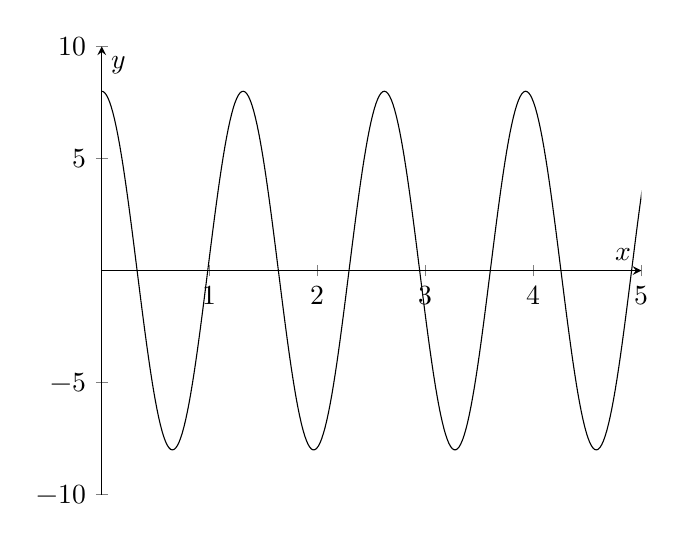
\begin{tikzpicture}
                            \begin{axis}[
                                axis lines = middle,
                                xmin = 0, xmax = 5,
                                ymin = -10, ymax = 10,
                                xlabel = $x$,
                                ylabel = {$y$},
                                samples = 800
                                ]
                                \addplot[domain=-2*pi:2*pi] {8 * sin(deg(4.8 * x + pi / 2))};
                            \end{axis}
                        \end{tikzpicture}
                    \end{figure}

                \item
                    Den skal være i \(]0,1[\) fordi den skal blive mindre og en eksponentialfunktion falder når
                    a er under 1.
                \item
                    Ligningen for amplituden er \(A(t) = 1 · a^{t}\). Amplituden er faldet fra 8 til 6 i 45 sekunder. 
                    \begin{align*}
                    A(45) &= \frac{6}{8} · a^{45} \\
                        a &= \left( \frac34\right)^{\frac{1}{45}} \approx 0,9936275
                   \end{align*}
                    \begin{figure}[htbp]
                        \centering
                        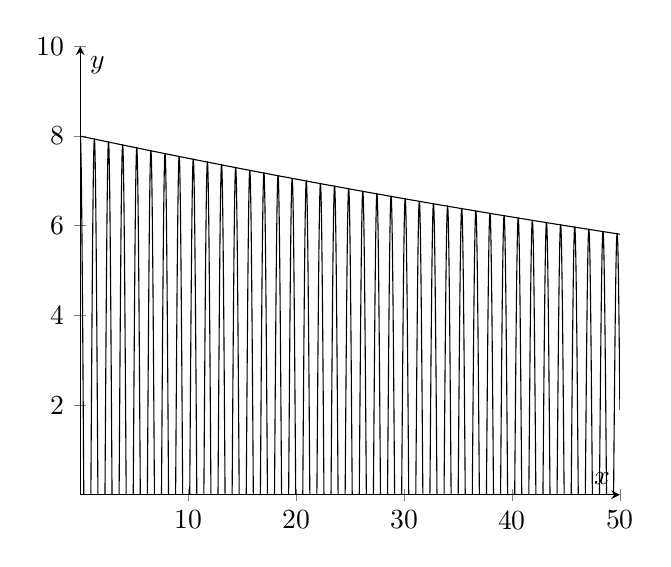
\begin{tikzpicture}
                            \begin{axis}[
                                axis lines = middle,
                                xmin = 0, xmax = 50,
                                ymin = 0, ymax = 10,
                                xlabel = $x$,
                                ylabel = {$y$},
                                samples = 10000
                                ]
                                \addplot[domain=0:50] {8*0.9936275^x};
                                \addplot[domain=0:50] {8*0.9936275^x *  sin(deg(4.8 * x + pi / 2))};
                            \end{axis}
                        \end{tikzpicture}
                    \end{figure}


                \item
                    Halveringstid er tid hvor funktionsværdien er halv så stort:
                    \begin{align*}
                        \left( \frac34\right)^{\frac{t}{45}} &= 1/2 \\
                        t &\approx 108,42
                    \end{align*}
                \item
                    Da fjederns udvidelse er afhængig af $A(t)$ skal vi find ud hvornår den er mindre end skal vi find ud
                    hvornår den er mindre end $3cm$. 
                    \begin{align*}
                        A(t) &= 8·\left( \frac34\right)^{\frac{t}{45}} = 3\\
                        t &\approx 153,42
                    \end{align*}
                    Det sker efter ca. 153 sekunder.
                \item
                    Her skal vi find afledningen af vores funktion og så skal vi se hvis den er positiv eller negativ:
                    \begin{align*}
                        f(t) &= \left( 8·\left( \frac34\right)^{\frac{t}{45}} \right) · \left(  \sin(4,8t+\fracπ2 \right)\\
                        f'(t) &= 2^{-\frac{2t}{45}}\, 3^{\frac{t}{45}}
\left(
    -0.0511435 \cos(4.8 t)
    - 38.4 \sin(4.8 t)
\right)\\
                        f'(153,42) &\approx -13,8148
                    \end{align*} 
                    Afledningen er negativ, det betyder at den er på vej ind.


                    Wolfram|Alpha blev brugt til de numeriske svar:\\
                    \href{https://www.wolframalpha.com/input?i=+derive+%28+8*%28+3%2F4%29%5E%7Bt%2F45%7D+%29+*+++sin%284.8t%2B%CF%80%2F2+%29+}{Afledning}\\
                    \href{https://www.wolframalpha.com/input?i=2%5E%28-%282+t%29%2F45%29+3%5E%28t%2F45%29+%28-0.0511435+cos%284.8+t%29+-+38.4+sin%284.8+t%29%29+where+t++%3D+153.42}{Indsætning af værdien}

            \end{enumerate}
    \end{enumerate}
\end{document}

